\begin{center}
    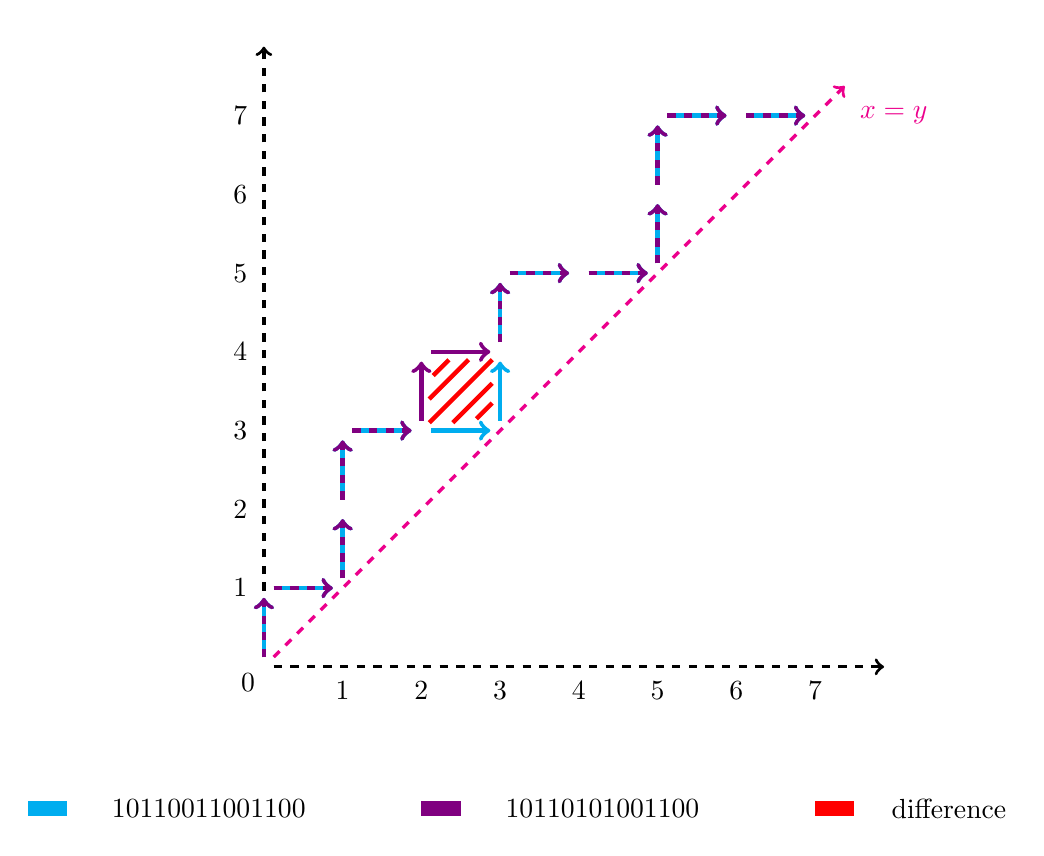
\begin{tikzpicture}[scale=1]
        \node (a) at (0, 0) {};
        \node (b) at (0, 8) {};
        \node (c) at (8, 0) {};
        \node (d) at (7.5, 7.5) {};
        \node (e) at (8, 7) [color = magenta]
            {$x = y$}; 
        \draw [dashed, very thick, ->] (a) to (b);
        \draw [dashed, very thick, ->] (a) to (c);
        \draw [dashed, very thick, ->]
            [color = magenta] (a) to (d);

        \node (1)  at (0,0)   {};
        \node (2)  at (0,1)   {};
        \node (3)  at (1,1)   {};
        \node (4)  at (1,2)   {};
        \node (5)  at (1,3)   {};
        \node (6)  at (2,3)   {};
        \node (7)  at (3,3)   {};
        \node (7b) at (2,4)   {};
        \node (8)  at (3,4)   {};
        \node (9)  at (3,5)   {};
        \node (10) at (4,5)   {};
        \node (11) at (5,5)   {};
        \node (12) at (5,6)   {};
        \node (13) at (5,7)   {};
        \node (14) at (6,7)   {};
        \node (15) at (7,7)   {};

        \draw [->, ultra thick, color = cyan]
            (1)  to (2);
        \draw [->, ultra thick, color = cyan] 
            (2)  to (3);
        \draw [->, ultra thick, color = cyan]
            (3)  to (4);
        \draw [->, ultra thick, color = cyan]
            (4)  to (5);
        \draw [->, ultra thick, color = cyan]
            (5)  to (6);
        \draw [->, ultra thick, color = cyan]
            (6)  to (7);
        \draw [->, ultra thick, color = cyan]
            (7)  to (8);
        \draw [->, ultra thick, color = cyan]
            (8)  to (9);
        \draw [->, ultra thick, color = cyan]
            (9)  to (10);
        \draw [->, ultra thick, color = cyan]
            (10) to (11);
        \draw [->, ultra thick, color = cyan]
            (11) to (12);
        \draw [->, ultra thick, color = cyan]
            (12) to (13);
        \draw [->, ultra thick, color = cyan]
            (13) to (14);
        \draw [->, ultra thick, color = cyan]
            (14) to (15);

        \draw [->, dashed, ultra thick, color = violet]
            (1)  to (2);
        \draw [->, dashed, ultra thick, color = violet] 
            (2)  to (3);
        \draw [->, dashed, ultra thick, color = violet]
            (3)  to (4);
        \draw [->, dashed, ultra thick, color = violet]
            (4)  to (5);
        \draw [->, dashed, ultra thick, color = violet]
            (5)  to (6);
        \draw [->, ultra thick, color = violet]
            (6)  to (7b);
        \draw [->, ultra thick, color = violet]
            (7b)  to (8);
        \draw [->, dashed, ultra thick, color = violet]
            (8)  to (9);
        \draw [->, dashed, ultra thick, color = violet]
            (9)  to (10);
        \draw [->, dashed, ultra thick, color = violet]
            (10) to (11);
        \draw [->, dashed, ultra thick, color = violet]
            (11) to (12);
        \draw [->, dashed, ultra thick, color = violet]
            (12) to (13);
        \draw [->, dashed, ultra thick, color = violet]
            (13) to (14);
        \draw [->, dashed, ultra thick, color = violet]
            (14) to (15);

        \node at (-0.2, -0.2) {$0$};
        \node at (-0.3, 1)    {$1$};
        \node at (1, -0.3)    {$1$};
        \node at (-0.3, 2)    {$2$};
        \node at (2, -0.3)    {$2$};
        \node at (-0.3, 3)    {$3$};
        \node at (3, -0.3)    {$3$};
        \node at (-0.3, 4)    {$4$};
        \node at (4, -0.3)    {$4$};
        \node at (-0.3, 5)    {$5$};
        \node at (5, -0.3)    {$5$};
        \node at (-0.3, 6)    {$6$};
        \node at (6, -0.3)    {$6$};
        \node at (-0.3, 7)    {$7$};
        \node at (7, -0.3)    {$7$};

        \draw[color = red, ultra thick]
            (2.1,3.1) -- (2.9,3.9);
        \draw[color = red, ultra thick]
            (2.1,3.4) -- (2.6,3.9);
        \draw[color = red, ultra thick]
            (2.15,3.7) -- (2.35,3.9);
        \draw[color = red, ultra thick]
            (2.4,3.1) -- (2.9,3.6);
        \draw[color = red, ultra thick]
            (2.7,3.15) -- (2.9,3.35);

        \fill[color = cyan] (-3,-1.9) rectangle
            (-2.5,-1.7);
        \node at (-0.7,-1.8) {$10110011001100$};
        \fill[color = violet] (2,-1.9) rectangle
        (2.5,-1.7);
        \node at (4.3,-1.8) {$10110101001100$};
        \fill[color = red] (7,-1.9) rectangle
        (7.5,-1.7);
        \node at (8.7,-1.8) {difference};
    \end{tikzpicture}
\end{center}